
\chapter{Автоматизация процесса проектирования путем генерации масштабируемого RTL-описания} \label{generation}

В данной главе описывается подход повышения эффективности процесса проектирования за счет автоматизации процесса генерации масштабируемого RTL-описания.

\section{Актуальность}

С увеличением количества интегрируемых IP-блоков в системах-на-кристалле (СнК), повышаются требования к узлам, отвечающим за их межсоединение.
Специфика разработки блоков межсоединения [более подробно в главе \ref{review}].

Необходимость создания параметризированного по количеству как ведомых (slave), так и ведущих (master) портов межсоединения повлекла за собой работу по созданию средств для генерации RTL-описания.

\section{Научная новизна}

Генерация выходного RTL-описания IP-блоков по заданным параметрам реализована у многих вендоров. У большинства из них этот процесс заключается в создании RTL-описания в соответсвие со специфическим синтаксисом, расширяющим стандартный язык описания аппаратуры (например, Synopsys CoreBuilder или открытый проект CONfigurable NEtwork Creation Tool). Такой подход является зависимым от конкретного вендора и может быть применен только для IP-блоков той фирмы, которая занимается их разработкой совместно с разработкой средств для генерации.

Также вопросом реализации автоматизации процесса создания конфигурируемых IP-блоков занимались и независимые от вендоров команды (например, CoreTML framework). При этом решая проблему зависимости от поставщика IP-блоков, они не снимают все ограничения с процесса генерации. Так, в основе решения задачи сохраняется необходимость написание RTL-кода согласно со специфическим синтаксисом, что привязывает описание к конкретному программному средству генерации.

Подход, который предложен в данной работе, решает сформулированные проблемы:

\begin{enumerate}
  \item Зависимость от вендора.
  \item Зависимость от средств генерации.
\end{enumerate}

\section{Генерация RTL-описания}

\subsection{Описание подхода}

\subsection{Парсинг входного RTL-описания}

Написана программа на языке с++, основная функциональная часть которой реализована на основе открытого программного обеспечения lex и yacc операционной системы Linux. Выполняется парсинг входного RTL-описания, на выходе получается XML-описание блока.

\subsection{Масштабирование}

Написана программа на языке go, работающая с XML-описанием блока, получаемого в результате парсинга. Дополнительными входными данными являются определяемые пользователем шаблоны, определяющие те участки кода, требующие масштабирования до значений, также указанных пользователем.

\subsection{Графический интерфейс}

Написана программа с графическим интерфейсом на языке c++ посредством Qt библиотеки, интегрирующая в себя этапы генерации RLT-описания по заданным параметрам, с дальнейшими этапами компиляции, симуляции и синтезом блока.

\begin{figure} [h]
  \center
  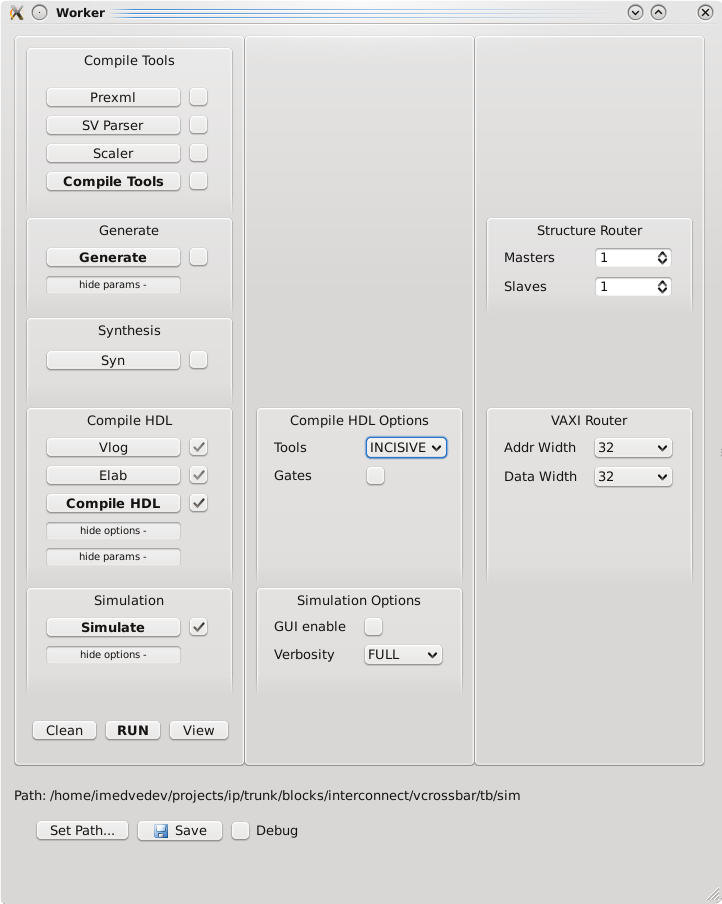
\includegraphics [scale=0.7] {pic01}
  \caption{Графический интерфейс программного средства генерации RTL-описания.}
  \label{img:pic01}
\end{figure}

\clearpage

